%!TEX root = IROS2019_DNN.tex

\begin{section}{Introduction} \label{sec:intro}

Autonomous vehicles are becoming increasingly popular and part of our daily lives. Autonomous transportation, package and food delivery, firefighting, law-enforcement, medical service, hobby, and house-hold applications are just some examples where the use of robotics is advantageous over other technologies. 

As they find their way into our society it becomes critical during run-time to guarantee safety against unpredictable uncertainties and disturbances. In fact, while model-driven motion planning and control techniques can be robust against noises and disturbances, they cannot prevent deviations from the desired behavior during the system operation which could potentially lead to unsafe states (e.g. crashing into an obstacle in the environment due to excessive wind disturbance). In order to assure safety of the autonomous operations, it is necessary to take the effect of noises and disturbances into consideration during planning. Traditional reachability analysis tools like \NB{CITE} have demonstrated to be very effective in predicting future states of the system by utilizing the knowledge about the system model and dynamics. However they are computationally expensive making them hard to use as run-time monitors, subject of this paper.

On the other hand machine learning provides a potentially innovative way to enable fast reachability analysis. Unfortunately, the lack of understanding of how machine learning works, makes it challenging to provide guarantees for autonomous systems in safety-critical operations.

To deal with these challenges, in this work we present a novel verified learning-enabled framework for fast run-time monitoring of autonomous systems. In our scheme, presented in Fig. ~\ref{fig:gen_app}  a verified deep neural network (DNN) is trained to recognize safe and unsafe trajectories for a quadrotor UAV in a obstacle populated environment. Training is performed by considering a library of trajectories and their associated reachable sets. A trajectory is labeled safe if its reachable tube doesn't collide with any obstacle while it is marked unsafe otherwise. Differently from most of the work in the literature, here we verify the validity of our trained DNN by using our recent tool VERISIG \cite{IvanovVerisig18} in which \NB{brief explanation about the tool}. 

At runtime, the verified and trained DNN is used to decide about the safety of a trajectory from an untrained initial state under the effect of noise and disturbance.
%will then decide if a new trajectory is safe or not under the effect of noise and disturbance. 
If unsafe, a new trajectory is computed by increasing the distance to keep from the obstacles in the environment and testing again for safety. 

%In the event that a trajectory is found unsafe, a new trajectory is computed by increasing the distance to keep from the obstacles in the environment and test

%Over the recent years, the autonomous vehicles have started to become a part of our daily lives. Package delivery robots, autonomous cars, hobby and service robots are just a few example of commonly used autonomous systems. As they become more commonplace, assuring the safety of autonomous operations gains even more importance.
%
%Even with the advanced control and planning algorithms, an autonomous system may reach unsafe states due to  uncertainties in real world such as disturbances, measurement and input noises. In order to assure the safety of the autonomous operations under these conditions, it is necessary to take the effect of noises and disturbances into consideration during planning. Traditional reachability tools are widely used to predict the future states of a hybrid system by utilizing the knowledge about system model and dynamics. Although they are powerful tools for assessing the safety of an autonomous system, they suffer from the curse of dimensionality. For hybrid systems with large state space, it becomes very challenging to analyze their reachability with traditional tools. 

%In this work, for assuring safety in autonomous operations at run-time, we introduce a verified machine learning based framework as presented in Fig.~\ref{fig:gen_app}. 
%At offline stage, various trajectories from different initial positions in the environment to a goal position are generated and the desired distance to keep from the obstacles (avoid distance) is specified by the user. The initial positions-avoid distance pairs are labeled as safe or unsafe based on the intersection of reachable sets with the obstacles in the environment. As a reachability tool, we use a simulation-based approach using the worst case scenario assumptions, but it should be noted that the general framework is independent of the choose of reachability tool. The set of safety labeled initial positions are then used to train a deep neural network (DNN) and the network is verified using the verification tool called Verisig \cite{IvanovVerisig18}. At the online stage, the verified and trained network is used in order to make decisions about the safety of a trajectory from an untrained initial position. If the planned trajectory is predicted to be safe, the plant can execute the trajectory, otherwise replanning is required.

\NB{the contribution needs to be fixed...I'll take care of this}The contribution of the proposed framework is twofold: 1) we assure the safety of an autonomous system regardless of the planning algorithm, 2) a verified safety decision is made fast at run-time. The proposed approach makes it possible to eliminate the need for the traditional and computational expensive reachability tools, as the proposed approach makes the same predictions as such tools would make in a much faster way.

The rest of the paper is organized as follows: In Section~\ref{sec:rel_lit} we give a review of related literature. We provide details about the system and controller models in Section~\ref{sec:model}, and we explain the proposed approach in details in Section~\ref{sec:method}. The proposed approach is validated with simulations and experiments in Sections~\ref{sec:simulation} and \ref{sec:experiment} respectively. Finally we draw conclusions and discuss about future work in Section~\ref{sec:conclusion}.

\begin{figure}[t]
	\centering
	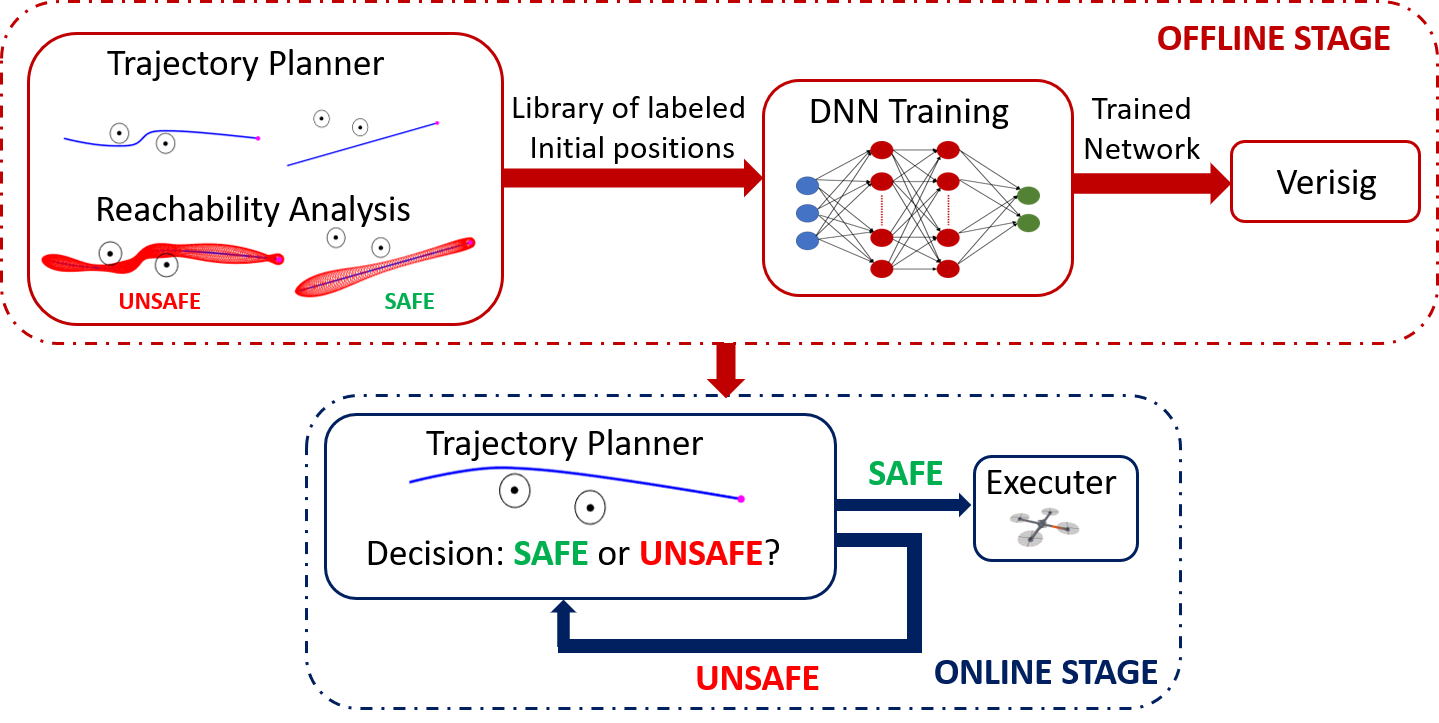
\includegraphics[width=0.45\textwidth]{figures/general_approach}
	\caption{General approach.} 
	\label{fig:gen_app}
\end{figure}
\NB{we need to change this figure. I don't like executer...let's use controller and plant instead}
\end{section}

